% Niveau :      PCSI *
% Discipline :  Chimie Orga I
% Mots clés :   Spectrométrie UV-visible, Réactions acidobasiques

\begin{exercise}{Méthode de Mohr}{2}{PCSI}
{Chimie générale,Réactions de précipitation,Mohr (méthode de),Titrage}{bermu}

Dans cet exercice, on étudie une solution de chlorure de sodium de concentration inconnue $c_0 \sim 10^{-2}$ M à l'aide d'une solution de nitrate d'argent.

\begin{questions}
\questioncours Critère de précipitation d'un solide en solution aqueuse. \\ On prendra l'exemple du chlorure d'argent.

\question Quelle est la solubilité $s_1$ du chlorure d'argent ?

\begin{EnvUplevel}
    On introduit dans un becher un volume $v_0 = 40,0$ mL de la solution que l'on souhaite titrer. Cette solution est titrée par une solution de nitrate d’argent de concentration $c_1 = 0,0250$ M.
    
    On considérera pour simplifier que la dilution est négligeable.
\end{EnvUplevel}

\question \'Ecrire la réaction support de titrage.

\question Sachant qu'une goutte délivrée par une burette a environ un volume $v_g \simeq 0,05$ mL, la réaction de titrage débute-t-elle dès la première goutte de nitrate d’argent versée ?

\question Définir l'équivalence et donner l'expression du volume équivalent $V_\text{eq}$ en fonction des données de l'exercice.

\begin{EnvUplevel}
    Afin de détecter expérimentalement cette équivalence, on ajoute dans la solution avant le titrage quelques gouttes d'une solution incolore de chromate de sodium Na$_2$CrO$_4$.
\end{EnvUplevel}

\question Sachant que les ions chromate sont susceptibles de donner avec les ions argent (I) un précipité rouge vif de chromate d’argent, calculer la concentration $c_2$ en ions chromate à apporter dans la solution initiale pour que l’apparition du précipité rouge se produise exactement à l’équivalence et permette ainsi de détecter celle-ci avec précision.

\question En quoi la précision du titrage serait-elle affectée si on introduisait au début du titrage une concentration 10 fois plus importante de chromate de sodium ? 10 fois moins ? Commenter.

\question On trouve suite à l'expérience $v_\text{eq} = 24$ mL. Quelle est la valeur de $c_0$ ? \\
Estimer l'incertitude sur cette valeur.

\end{questions}

\paragraph{Données : }~\\
AgC$\ell$ \quad p$K_{s1} = 9,8$, \\
Ag$_2$CrO$_4$ \quad p$K_{s2} = 12,0$.


\end{exercise}

\newpage

\begin{solution}
\begin{questions}
    \questioncours La réaction $\mathrm{AgC\ell_\text{s} \leftrightharpoons {Ag^+}_\text{aq} + {C\ell^-}_\text{aq}}$ admet pour constante d'équilibre $K_{s1}$. Le solide n'existe que pour $Q_{r1} > K_{s1}$ :
    \begin{center}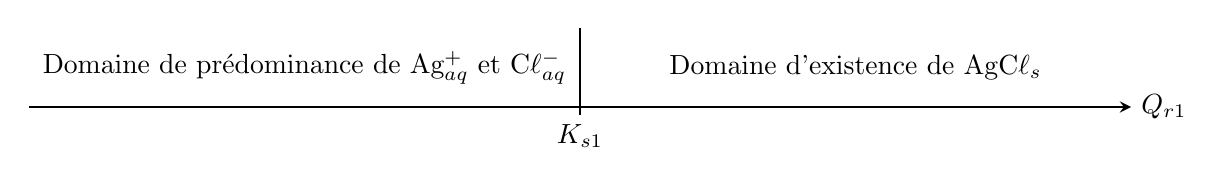
\begin{tikzpicture}[baseline=1em]
        \draw[->, >=stealth, thick] (-7,0)--(7,0) node[right]{$Q_{r1}$};
        \draw[black] (0,1)--(0,-0.1) node[below]{$K_{s1}$} ;
        \node at (-3.5,.5) {Domaine de prédominance de Ag$^+_\text{aq}$ et C$\ell^-_\text{aq}$};
        \node at (3.5,.5) {Domaine d'existence de AgC$\ell_\text{s}$};
    \end{tikzpicture}\end{center}
    
    \question On suppose qu'on introduit une quantité grande de AgC$\ell$ dans de l'eau pure. \`A l'équilibre
    $$K_{s1} = \mathrm{[Ag^+][C\ell^-]} = s^2,$$
    donc $s = 10^{-\text{p}K_{s1}/2} = 1,3 \times 10^{-5}$ M.
    
    \question La réaction est
    $$\mathrm{{Ag^+}_\text{aq} + {C\ell^-}_\text{aq} \longrightarrow AgC\ell_\text{s}}$$
    
    \question Au début, [Ag$^+$] $= 0$.
    \`A la première goutte, [Ag$^+$]$ = \dfrac{c_1 v_g}{v_0}$ donc
    $$Q_{r1} = c_0 c_1 \dfrac{v_g}{v_0} > K_{s1} \qqtext{ou} c_0 > \dfrac{K_{s1} v_0}{c_1 v_g} \simeq 5,1 \times 10^{-6} \text{ M},$$
    le précipité apparaît donc dès la première goutte de titrant versée si la concentration $c_0$ est supérieure à $5,1 \times 10^{-6}$ M.
    
    \question Par définition, l’équivalence est obtenue lorsqu’on a apporté Ag$^+$ et C$\ell^-$ dans les proportions st{\oe}chiométriques de la réaction de titrage, ici 1:1, soit
    $$n_\text{eq} = n_\mathrm{C\ell^-} = n_\mathrm{Ag^+} \qquad \Longleftrightarrow \qquad c_0 v_0 = c_1 v_\text{eq}.$$
    
    \question \`A l’équivalence le titrant a consommé exactement le titré : la réaction est quasi-totale. Il ne reste donc qu'une trace d'ions Ag$^+$ et C$\ell^-$, égale à la solubilité $s$ calculée à la question 2.
    
    Si on veut que la solution devienne saturée en Ag$_2$CrO$_4$ à l'équivalence, il faut que la concentration en CrO$_4^{2-}$, $c_2$ soit telle que 
    $$Q_{r2} = \mathrm{[Ag^+]^2 [CrO_4^{2-}]} = s^2 c_2 > K_{s2} \qqtext{ou} c_2 = \dfrac{K_{s2}}{K_{s1}} = 6,3 \times 10^{-3} \text{ M}.$$
    
    \question Si on apporte $\gamma$ (10 ou 1/10) plus de fois d’ions chromate, $\mathrm{[CrO_4^{2-}]} = \gamma c_2$, le précipité Ag$_2$CrO$_4$ va apparaître (avant l'équivalence si $\gamma > 1$ et après si $\gamma < 1$) lorsque
    $$\mathrm{[Ag^+]}_\text{seuil} = \sqrt{\dfrac{K_{s2}}{\gamma c_2}} = \sqrt{\dfrac{K_{s1}}{\gamma}},$$
    et donc quand
    $$\mathrm{[Cl^-]}_\text{seuil} = \dfrac{K_s}{\mathrm{[Ag^+]}} = \dfrac{s}{\sqrt{\gamma}},$$
    ce qui génère une erreur sur le volume équivalent de l'ordre de
    $$\dfrac{\mathrm{[Cl^-]}_\text{seuil} - c_0}{c_0} = (\gamma^{-1/2} - 1)s/c_0$$
    Ainsi l'erreur est très faible et la concentration $c_2$ a peu d'influence sur le résultat.
    
    \question On trouve
    $$c_0 = \dfrac{c_1 v_\text{eq}}{v_0} = 0,015 \text{ M}.$$

\end{questions}
\end{solution}